\documentclass[tikz, border=10pt]{standalone}
\usepackage{tikz}
\usetikzlibrary{calc,patterns}

\begin{document}
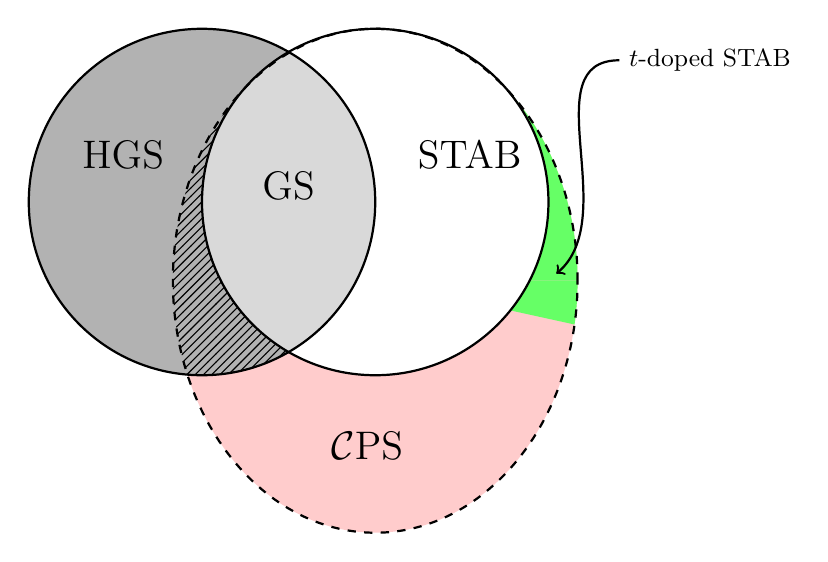
\begin{tikzpicture}[font=\Large]
\def\r{2.2}

\coordinate (CHGS)  at (-1.1, 1.0);
\coordinate (CSTAB) at ( 1.1, 1.0);
\coordinate (CCPS)  at ( 1.1, 0.0);

% New ellipse center (same as CPS here)
\coordinate (CGREEN) at (1.1,0.0);

% CPS ellipse radii
\def\cpsx{2.57}
\def\cpsy{3.2}

% --- Base fills ---
% CPS
\fill[pink!80] (CCPS) ellipse (\cpsx cm and \cpsy cm);

% Half-green ellipse on top of CPS (no border)
\fill[green!60]
  ($(CGREEN)+(\cpsx,0)$)
  arc[start angle=0,end angle=-10,
      x radius=\cpsx cm,
      y radius=\cpsy cm]
  -- (CGREEN) -- cycle;
\fill[green!60]
  ($(CGREEN)+(\cpsx,0)$)
  arc[start angle=0,end angle=180,
      x radius=\cpsx cm,
      y radius=\cpsy cm]
  -- (CGREEN) -- cycle;

% STAB
\fill[white] (CSTAB) circle (\r);

% HGS
\fill[gray!60] (CHGS) circle (\r);

% --- Intersections ---
% GS = HGS ∩ STAB
\begin{scope}
  \clip (CHGS) circle (\r);
  \fill[gray!30] (CSTAB) circle (\r);
\end{scope}

% HGS ∩ CPS without GS
\begin{scope}
  \clip (CHGS) circle (\r);
  \clip (CCPS) ellipse (\cpsx cm and \cpsy cm);

  \fill[
    pattern=north east lines,
    pattern color=black,
    even odd rule
  ]
    (CHGS) circle (\r)
    (CSTAB) circle (\r);
\end{scope}

% --- Outlines ---
\draw[thick] (CHGS) circle (\r);
\draw[thick] (CSTAB) circle (\r);

\draw[thick,dashed]
  (CCPS) ellipse (\cpsx cm and \cpsy cm);

% % Outline of half-green ellipse
% \draw[thick,green!70!black]
%   ($(CGREEN)+(\cpsx,0)$)
%   arc[start angle=0,end angle=180,
%       x radius=\cpsx cm,
%       y radius=\cpsy cm];

% --- Annotation for green region ---
\draw[->, thick]
  (4.2,2.8) 
  to[out=180,in=40]
  (3.4,.09);

\node[right] at (4.2,2.8) {\small $t$-doped STAB};

% --- Labels ---
\node at (-2.1, 1.6) {HGS};
\node at ( 2.3, 1.6) {STAB};
\node at ( 0.0, 1.2) {GS};
\node at ( 1.0,-2.1) {$\mathcal{C}$PS};

\end{tikzpicture}
\end{document}